\chapter{Solution Design and Architecture}
\label{chap:solution_design}

% ── chapter-local helpers ─────────────────────────────────────────────
\providecommand{\code}[1]{\texttt{\detokenize{#1}}}
\newcolumntype{F}[1]{>{\footnotesize\raggedright\arraybackslash}p{#1}}
\newcolumntype{C}[1]{>{\footnotesize\centering\arraybackslash}p{#1}}
\setlength{\LTcapwidth}{\textwidth}
\sloppy
% image slot: shows the image if the file exists, otherwise an empty frame
% with the expected file name (drop the file there and recompile)
\providecommand{\imgslot}[3]{\IfFileExists{#1}{\includegraphics[width=#2]{#1}}%
  {\fbox{\parbox[c][#3][c]{\dimexpr#2-2\fboxsep-2\fboxrule\relax}{\centering\color{gray}\footnotesize\texttt{\detokenize{#1}}}}}}
% start a new page only if less than #1 of vertical space is left
% (keeps a section title together with its full-page diagram)
\makeatletter
\providecommand{\keepwith}[1]{\par\begingroup\setlength{\dimen@}{#1}%
  \dimen@ii\pagegoal\advance\dimen@ii-\pagetotal
  \ifdim\dimen@>\dimen@ii\ifdim\dimen@ii>\z@\vfil\fi\break\fi\endgroup}
\makeatother

% ─────────────────────────────────────────────
\section*{Introduction}
\addcontentsline{toc}{section}{Introduction}
% ─────────────────────────────────────────────

This chapter presents the design of the Talently platform. It first describes the global architecture of the solution, then details its two core components, the SAP BTP ABAP RAP backend and the AI evaluation microservice, before presenting the user interfaces and the detailed design through class and sequence diagrams.

\newpage

% ═══════════════════════════════════════════════
\section{Application Architecture}
\label{sec:application_architecture}
% ═══════════════════════════════════════════════

% ──────────────────────────────────────────────
\subsection{Global System Architecture}
\label{subsec:global_architecture}
% ──────────────────────────────────────────────

Talently follows a modular and decoupled architecture that respects SAP's Clean Core principle: all business data and rules live in an SAP BTP extension, while the AI processing runs in a separate microservice. Figure~\ref{fig:global_architecture} gives an overview of the solution.

\begin{figure}[htbp]
    \centering
    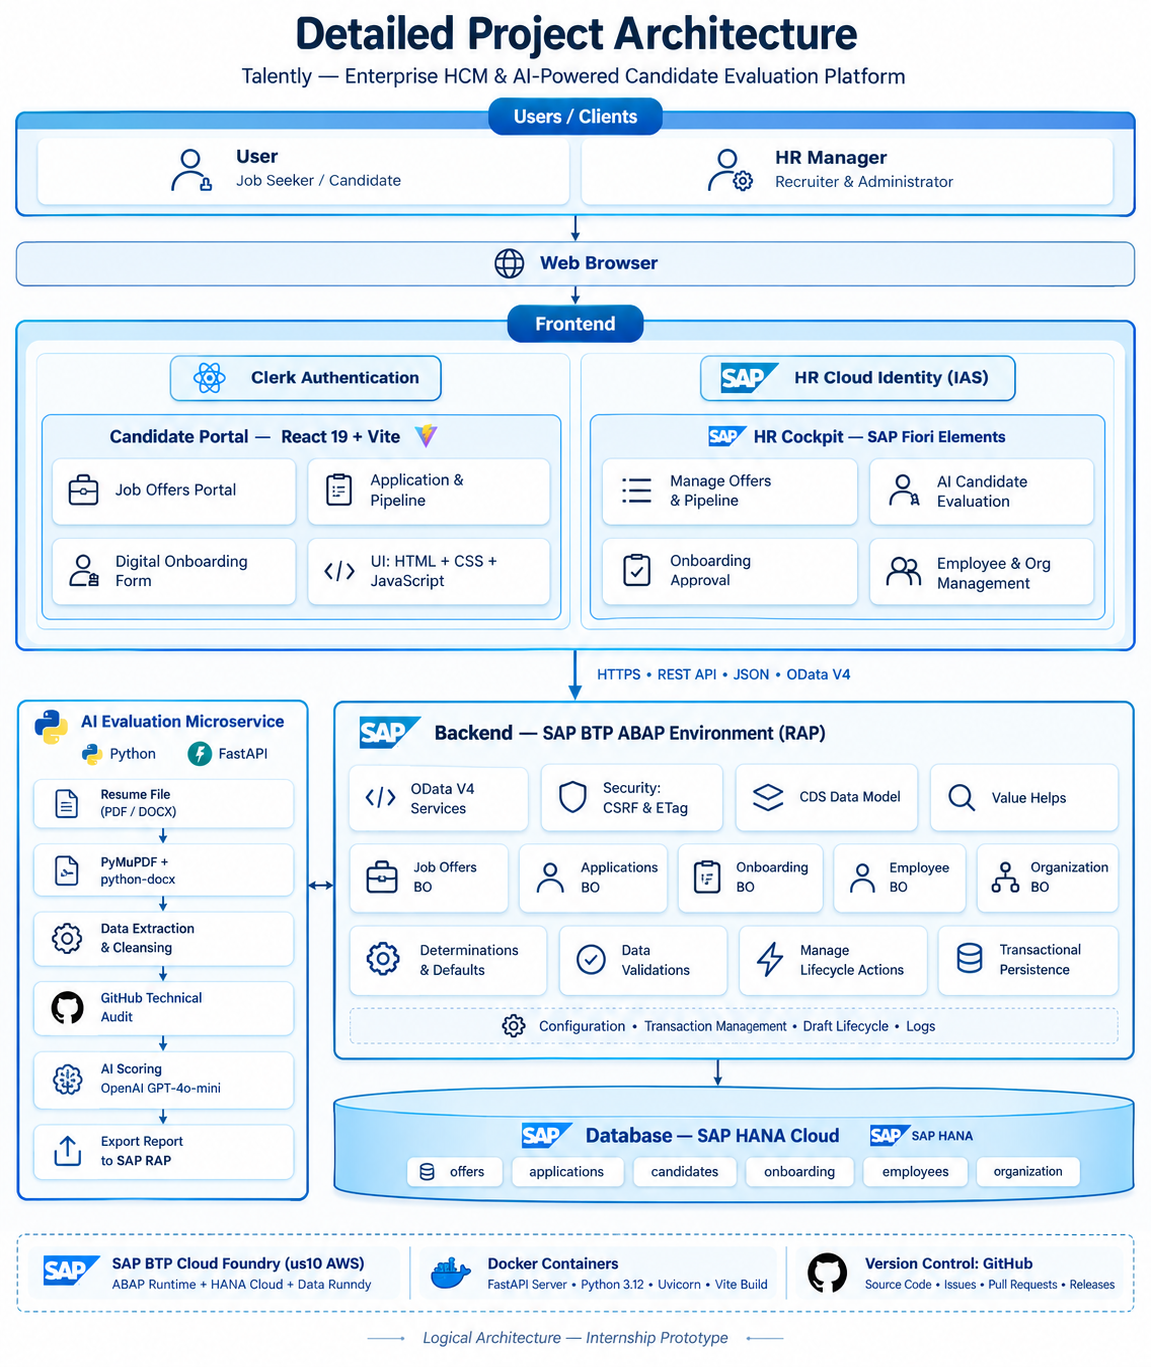
\includegraphics[width=0.78\textwidth]{Figures/global_architecture.png}
    \caption{Global System Architecture of the Talently Platform}
    \label{fig:global_architecture}
\end{figure}

\begin{itemize}
    \item \textbf{Users:} two profiles access the platform through a web browser: the \emph{candidate} (job seeker) and the \emph{HR manager} (recruiter and administrator).
    \item \textbf{Frontend:} two separate portals, each with its own identity provider. The \textbf{candidate portal} (React 19 + Vite) offers the job board, the application and pipeline tracking, and the onboarding form, with authentication handled by \textbf{Clerk}. The \textbf{HR cockpit} (SAP Fiori Elements) offers offer and pipeline management, AI candidate evaluation, onboarding approval, and employee and organization management, with authentication handled by \textbf{SAP Cloud Identity Services (IAS)}.
    \item \textbf{Backend (SAP BTP ABAP Environment, RAP):} the system of record. It exposes OData V4 services protected by CSRF tokens and ETags, and implements the five business domains (job offers, applications, onboarding, employees, and organization) as RAP business objects with determinations, validations, and lifecycle actions.
    \item \textbf{AI evaluation microservice (Python, FastAPI):} analyzes resumes, audits the candidate's GitHub activity, scores the candidate with GPT-4o-mini, and returns the result to the portal, which writes it to the backend.
    \item \textbf{Database (SAP HANA Cloud):} stores the active and draft records of all HR domains.
    \item \textbf{Infrastructure:} SAP BTP Cloud Foundry (us10 region) hosts the ABAP runtime and HANA Cloud, the FastAPI service is packaged as a Docker image, and GitHub manages the source code. In the prototype, the AI microservice and the candidate portal run on the development machine, the portal through the Vite development server and its proxy.
\end{itemize}

All exchanges use HTTPS and JSON: REST for the AI microservice and OData V4 for the SAP backend.

The end-to-end flow is as follows. A candidate applies through the portal, and the application is stored in SAP. The resume is sent to the AI microservice, whose score is written back to the application. The recruiter reviews the candidate in the Fiori cockpit, moves them through the pipeline, and accepts them. The candidate then completes the onboarding form, and its approval by HR creates the employee master record in a single RAP transaction, without any manual re-entry.

% ──────────────────────────────────────────────
\subsection{Simplified Backend Architecture}
\label{subsec:backend_architecture}
% ──────────────────────────────────────────────

The backend is built with the ABAP RESTful Application Programming Model (RAP)~\cite{sap_rap} on the SAP BTP ABAP Environment~\cite{sap_btp_abap}, using the \emph{managed scenario with draft}. In this scenario, the developer declares the data model and the business rules, while the SAP framework handles request processing, transactional buffering, locking, draft storage, and database access. Figure~\ref{fig:backend_architecture} shows the four layers of the backend.

\begin{figure}[htbp]
    \centering
    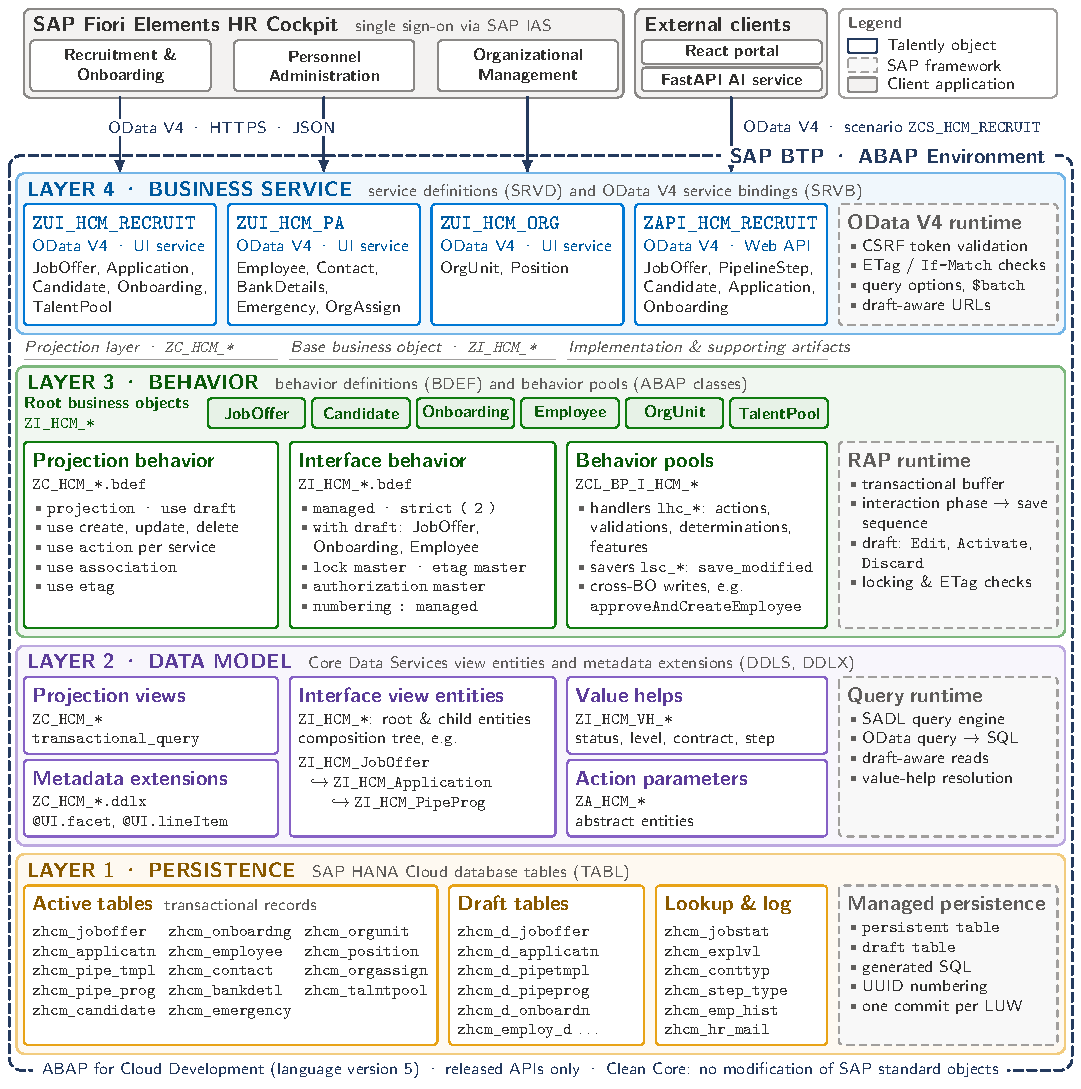
\includegraphics[width=\textwidth]{Figures/backend_architecture.pdf}
    \caption{ABAP RAP Backend -- Four-Layer Architecture}
    \label{fig:backend_architecture}
\end{figure}

\begin{itemize}
    \item \textbf{Business service layer:} service definitions (SRVD) and OData V4~\cite{odata} service bindings (SRVB). Three UI services serve the Fiori cockpit (\code{ZUI_HCM_RECRUIT}, \code{ZUI_HCM_PA}, \code{ZUI_HCM_ORG}), and one Web API, \code{ZAPI_HCM_RECRUIT}, is published through the communication scenario \code{ZCS_HCM_RECRUIT} for external integrations. In the prototype, the candidate portal calls the recruitment service \code{ZUI_HCM_RECRUIT} through a development proxy, both for the applications and for writing back the AI results.
    \item \textbf{Behavior layer:} behavior definitions (BDEF) declare, for each business object, its operations, actions, validations, determinations, locking, ETag, and draft handling (\code{managed}, \code{strict ( 2 )}, \code{with draft}). The logic is implemented in behavior pools (\code{ZCL_BP_I_HCM_*}), split into handler classes (\code{lhc_*}) and saver classes (\code{lsc_*}).
    \item \textbf{Data model layer:} Core Data Services (CDS) view entities~\cite{sap_cds}. Interface views (\code{ZI_HCM_*}) define the canonical data model and its compositions, projection views (\code{ZC_HCM_*}) adapt it to each service, and metadata extensions carry the Fiori UI annotations.
    \item \textbf{Persistence layer:} SAP HANA Cloud tables: active tables (\code{zhcm_joboffer}, \code{zhcm_applicatn}, \code{zhcm_employee}, \ldots), draft tables (\code{zhcm_d_joboffer}, \ldots), and lookup and log tables (\code{zhcm_jobstat}, \code{zhcm_emp_hist}, \ldots).
\end{itemize}

The dashed boxes of Figure~\ref{fig:backend_architecture} show what the SAP framework provides at each layer (CSRF and ETag checks, transactional buffer, query engine, SQL generation), so the Talently code contains only business rules. The backend is written in ABAP for Cloud Development using released APIs only, so no SAP standard object is modified.

\paragraph*{Business objects.} Table~\ref{tab:bo_catalogue} lists the six business objects of the backend. A child entity is created, locked, and saved together with its root: for example, an application belongs to its job offer, so locking an offer protects its whole recruitment pipeline. The candidate, the onboarding form, and the employee are separate roots because each has its own lifecycle. Draft handling is enabled only for the objects that HR users edit in several steps, and all keys are UUIDs generated by the framework.

\begingroup
\linespread{1}\selectfont
\renewcommand{\arraystretch}{1.4}
\begin{longtable}{@{}F{3.6cm}F{7.9cm}C{1.1cm}F{4.6cm}@{}}
\caption{Business Objects of the Talently Backend}\label{tab:bo_catalogue}\\
\toprule
\textbf{Business object} & \textbf{Child entities} & \textbf{Draft} & \textbf{Service} \\
\midrule
\endfirsthead
\toprule
\textbf{Business object} & \textbf{Child entities} & \textbf{Draft} & \textbf{Service} \\
\midrule
\endhead
\bottomrule
\endlastfoot
\code{ZI_HCM_OrgUnit} & \code{ZI_HCM_Position} & Yes & \code{ZUI_HCM_ORG} \\
\code{ZI_HCM_JobOffer} & \code{ZI_HCM_PipeTmpl}, \code{ZI_HCM_Application} $\rightarrow$ \code{ZI_HCM_PipeProg} & Yes & \code{ZUI_HCM_RECRUIT}, \code{ZAPI_HCM_RECRUIT} \\
\code{ZI_HCM_Candidate} & -- & No & \code{ZUI_HCM_RECRUIT}, \code{ZAPI_HCM_RECRUIT} \\
\code{ZI_HCM_Onboarding} & -- & Yes & \code{ZUI_HCM_RECRUIT}, \code{ZAPI_HCM_RECRUIT} \\
\code{ZI_HCM_Employee} & \code{ZI_HCM_Contact}, \code{ZI_HCM_BankDetl}, \code{ZI_HCM_Emergency}, \code{ZI_HCM_OrgAssign} & Yes & \code{ZUI_HCM_PA} \\
\code{ZI_HCM_TalentPool} & -- & No & \code{ZUI_HCM_RECRUIT} \\
\end{longtable}
\endgroup

\paragraph*{Main business actions.} Table~\ref{tab:main_actions} summarizes the main actions. Their availability is computed for each instance (feature control): for example, \emph{Publish} is only enabled for a draft or closed offer, and \emph{Accept to Post} only when the candidate has reached the last pipeline step. In addition, validations block inconsistent data before it is saved: mandatory fields, application deadline, vacant position, duplicate applications, and at least one pipeline step before publishing.

\begingroup
\linespread{1}\selectfont
\renewcommand{\arraystretch}{1.4}
\begin{longtable}{@{}F{5.6cm}F{2.8cm}F{9.1cm}@{}}
\caption{Main Business Actions of the Backend}\label{tab:main_actions}\\
\toprule
\textbf{Action} & \textbf{Business object} & \textbf{Effect} \\
\midrule
\endfirsthead
\toprule
\textbf{Action} & \textbf{Business object} & \textbf{Effect} \\
\midrule
\endhead
\bottomrule
\endlastfoot
\code{publishOffer}, \code{closeOffer} & Job offer & Publishes the offer on the portal or closes it. \\
\code{applyToJob} & Candidate & Creates an application at the first pipeline step. \\
\code{setAIEvaluation}, \code{evaluateWithAI} & Application & Stores the AI score, recommendation, and summary, or flags the application for a new evaluation (\emph{PENDING}). \\
\code{passToNextStep} & Application & Moves the candidate to the next pipeline step. \\
\code{acceptToPost} & Application & Accepts the candidate, prepares the onboarding form, and closes the offer when all positions are filled. \\
\code{rejectCandidate} & Application & Rejects the candidate and adds them to the talent pool. \\
\code{approveAndCreateEmployee} & Onboarding & Creates the employee master record with contact, bank, emergency, and assignment data. \\
\code{promoteEmployee}, \code{transferEmployee}, \code{terminateEmployee} & Employee & Records personnel events in the employment history. \\
\end{longtable}
\endgroup

\paragraph*{Transaction model.} RAP executes every request in two phases. During the \emph{interaction phase}, the handler classes apply the changes to an in-memory transactional buffer. During the \emph{save sequence}, all validations run; if they pass, the buffer is written and committed as a single database transaction, otherwise nothing is saved. Because RAP forbids database writes during the interaction phase, the records of other business objects are written by the saver classes during the save sequence, following a \emph{buffer-then-save} pattern. For example, \code{approveAndCreateEmployee} buffers the form data, and the saver class \code{lsc_ZI_HCM_ONBOARDING} creates the employee during the save sequence. The hiring is therefore atomic: either the employee record is fully created and the form approved, or nothing changes.

\keepwith{0.9\textheight}
\subsubsection{Sequence Diagram: Job Offer Management}
\label{subsubsec:seq_job_offer}

\begin{figure}[H]
    \centering
    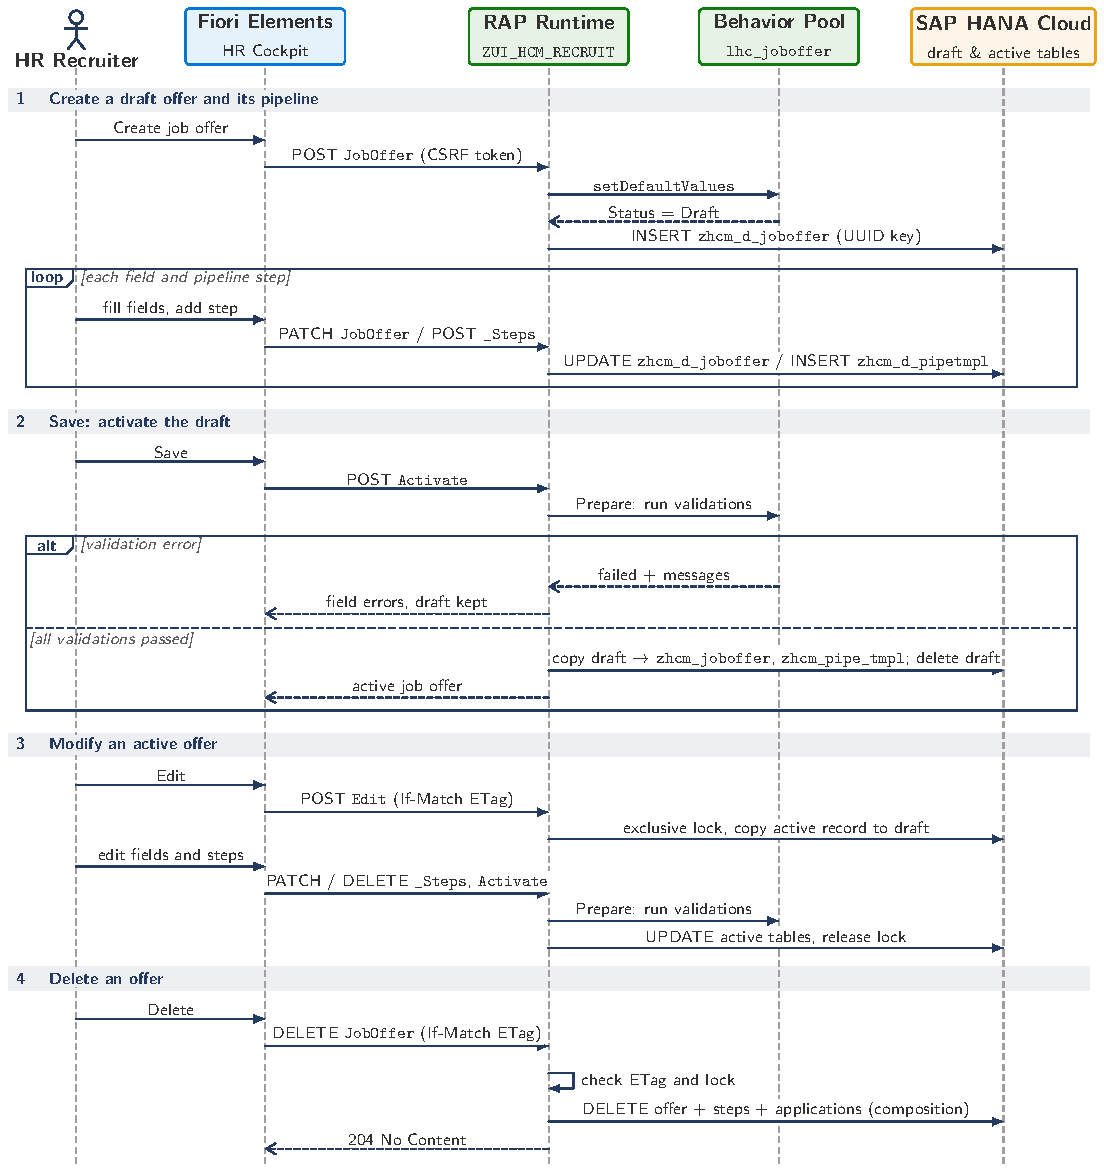
\includegraphics[width=\textwidth]{Figures/seq_job_offer.pdf}
    \caption{Sequence Diagram -- Job Offer Management (Create, Modify, Delete)}
    \label{fig:seq_job_offer}
\end{figure}

The diagram follows the four operations of a recruiter on a job offer:

\begin{enumerate}
    \item \textbf{Create:} the RAP runtime creates a draft with a UUID key and the status \emph{Draft}; the fields and pipeline steps are saved automatically in the draft tables.
    \item \textbf{Save:} the \emph{Activate} action runs the validations. On error, the draft is kept; otherwise, the offer and its steps are copied to the active tables in one transaction.
    \item \textbf{Modify:} the \emph{Edit} action locks the offer and copies it into a new draft, so two recruiters cannot change it at the same time.
    \item \textbf{Delete:} protected by the ETag, it removes the offer together with its pipeline steps and applications (composition).
\end{enumerate}

% ──────────────────────────────────────────────
\subsection{Simplified AI Agent Architecture}
\label{subsec:ai_architecture}
% ──────────────────────────────────────────────

The AI evaluation engine is a stateless Python microservice built with FastAPI. It is kept outside SAP so that slow or unpredictable LLM processing never affects ERP transactions. It receives a resume together with the target job offer, and returns a structured, explainable score. Figure~\ref{fig:ai_engine} shows its processing pipeline.

\begin{figure}[htbp]
    \centering
    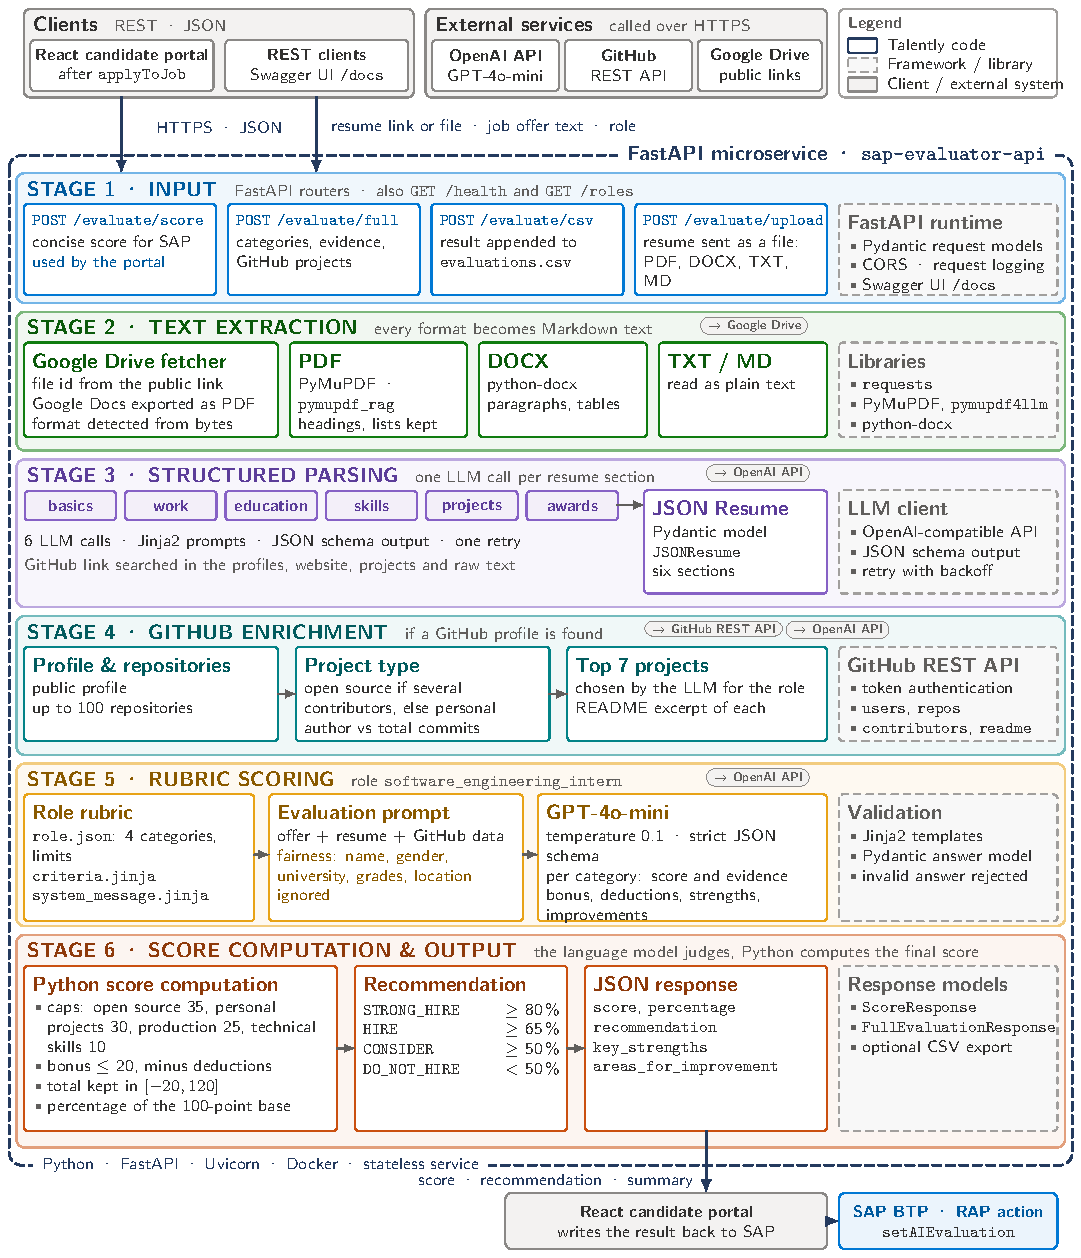
\includegraphics[width=0.97\textwidth]{Figures/ai_evaluation_engine.pdf}
    \caption{AI Evaluation Microservice -- Resume Scoring Pipeline}
    \label{fig:ai_engine}
\end{figure}

The pipeline runs in six stages:

\begin{enumerate}
    \item \textbf{Input:} the resume is received as a Google Drive link or an uploaded file (PDF, DOCX, TXT, or MD), together with the job offer description, through the REST endpoints \code{/evaluate/score} and \code{/evaluate/full}.
    \item \textbf{Text extraction:} the document is downloaded from Google Drive (or received as a file) and converted into clean Markdown (PyMuPDF for PDF, python-docx for Word).
    \item \textbf{Structured parsing:} six LLM calls extract the basics, work experience, education, skills, projects, and awards into the standard JSON Resume model~\cite{jsonresume}, validated with Pydantic.
    \item \textbf{GitHub enrichment:} the candidate's GitHub profile is detected automatically. The GitHub API~\cite{github_api} provides the repositories and commit statistics, each project is classified as open source or personal, the LLM selects the seven most relevant ones, and their README quality is checked.
    \item \textbf{Rubric scoring:} GPT-4o-mini (temperature 0.1) evaluates the candidate against the rubric of the target role, defined in Jinja2 templates, and against the text of the job offer. The text sent to the model contains no personal identifiers: the name, contact details, location, institution, and grades are left out. The model must answer in a strict JSON schema~\cite{openai_structured} with evidence for each category, key strengths, and areas for improvement.
    \item \textbf{Score computation and write-back:} the final score is computed in Python (category caps, bonus, deductions, and a total bounded to $[-20, 120]$), a recommendation is derived, and the result is returned to the portal, which writes it to the application in SAP through the RAP action \code{setAIEvaluation}.
\end{enumerate}

\begingroup
\linespread{1}\selectfont
\renewcommand{\arraystretch}{1.4}
\begin{longtable}{@{}F{13.5cm}C{4.0cm}@{}}
\caption{Evaluation Rubric of the Software Engineering Intern Role}\label{tab:ai_rubric}\\
\toprule
\textbf{Criterion} & \textbf{Points} \\
\midrule
\endfirsthead
\toprule
\textbf{Criterion} & \textbf{Points} \\
\midrule
\endhead
\midrule
\multicolumn{2}{@{}F{17.5cm}@{}}{Recommendation: \textbf{STRONG\_HIRE} ($\geq$ 80\,\%), \textbf{HIRE} ($\geq$ 65\,\%), \textbf{CONSIDER} ($\geq$ 50\,\%), \textbf{DO\_NOT\_HIRE} ($<$ 50\,\%).} \\
\bottomrule
\endlastfoot
Open source contributions & 0 -- 35 \\
Personal projects & 0 -- 30 \\
Production experience & 0 -- 25 \\
Technical skills & 0 -- 10 \\
Bonus (e.g., Google Summer of Code, startup experience, portfolio) & up to +20 \\
Deductions (e.g., tutorial-only projects, projects without links or README) & $-N$ \\
\end{longtable}
\endgroup

Two design choices make the evaluation trustworthy. First, the LLM judges but Python calculates: the final number is computed deterministically from the LLM's structured answer, so it always respects the rubric limits. Second, the evaluation is designed to be fair: the prompt forbids using the candidate's name, gender, university, grades, or location, and these details are not even sent to the scoring model. This second measure was added after the fairness test presented in Chapter~\ref{chap:implementation}. The score only supports the recruiter, who keeps the final decision in the Fiori cockpit.

\keepwith{0.8\textheight}
\subsubsection{Sequence Diagram: Candidate Application and AI Evaluation}
\label{subsubsec:seq_ai_evaluation}

\begin{figure}[H]
    \centering
    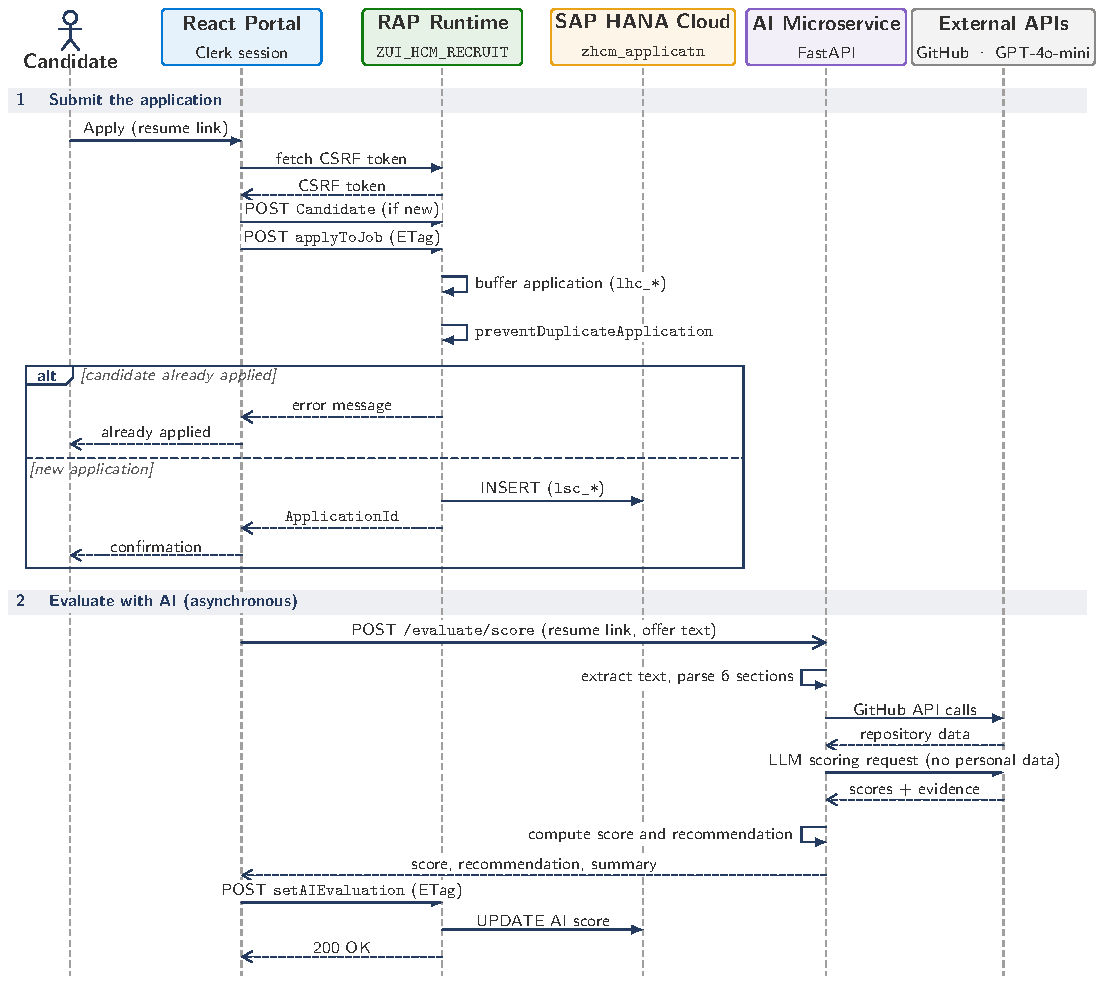
\includegraphics[width=\textwidth]{Figures/seq_ai_evaluation.pdf}
    \caption{Sequence Diagram -- Candidate Application and AI Evaluation}
    \label{fig:seq_ai_evaluation}
\end{figure}

The scenario runs in two phases:

\begin{enumerate}
    \item \textbf{Application:} the portal obtains a CSRF token and calls \code{applyToJob} on the service \code{ZUI_HCM_RECRUIT}. The application is inserted only if the duplicate-application check passes.
    \item \textbf{AI evaluation:} the portal sends the resume link and the offer text to the AI microservice asynchronously, so the candidate does not wait. The service parses the resume, queries GitHub and GPT-4o-mini, and computes the score; the portal then writes the result back through \code{setAIEvaluation}, where it becomes visible to the recruiter in the Fiori cockpit.
\end{enumerate}

% ──────────────────────────────────────────────
\subsection{UI/UX Expectations}
\label{subsec:uiux}
% ──────────────────────────────────────────────

Talently has two interfaces for two audiences. The candidate portal is a free React design focused on simplicity and self-service, while the HR cockpit follows the SAP Fiori design guidelines~\cite{sap_fiori_design}: its screens are generated by SAP Fiori Elements~\cite{sap_fiori_elements} from the annotations of the CDS projection views, using the standard \emph{List Report} and \emph{Object Page} floorplans. Figure~\ref{fig:routing_tree} shows the navigation of both interfaces.

\begin{figure}[H]
\centering
\begin{minipage}{0.97\textwidth}
\linespread{1}\selectfont\footnotesize
\begin{verbatim}
Candidate Portal (React 19, React Router)
/                     Job Board: published offers, search and filters
|-- /jobs/:id         Job Details: description, skills, pipeline steps, apply form
|-- /applications     My Applications: offers applied to, progress tracking
|-- /onboarding/:id   Onboarding Form: personal, legal, bank and emergency data
|-- /talent-pool      Talent Pool: non-selected candidates (HR role only)
`-- *                 Fallback page
Sign-in / Sign-up     Clerk modal, available from every page

HR Cockpit (SAP Fiori Elements: List Report -> Object Page)
Recruitment & Onboarding  (ZUI_HCM_RECRUIT)
|-- Job Offers -> Job Offer: General Information, Pipeline Steps, Applications
|   `-- Application: details, AI score, Pipeline Progress
|-- Onboarding Forms -> Onboarding Form: personal, bank and legal data
`-- Talent Pool
Personnel Administration  (ZUI_HCM_PA)
`-- Employees -> Employee: Contact, Bank Details, Emergency, Assignment
Organizational Management (ZUI_HCM_ORG)
`-- Organizational Units -> Organizational Unit: Positions
\end{verbatim}
\end{minipage}
\caption{Application Routing Tree of the Candidate Portal and the HR Cockpit}
\label{fig:routing_tree}
\end{figure}

The main screens were first sketched as low-fidelity wireframes with Excalidraw, which fixed the layout of each screen and the information it shows. The sketches were then refined into higher-fidelity mockups. Figure~\ref{fig:wireframes_portal} shows the mockup of the job board of the candidate portal, with its four zones: navigation header, search and filter bar, filter sidebar, and job card. Figure~\ref{fig:wireframes_cockpit} shows the mockup of the job offers list of the HR cockpit, built on the standard Fiori List Report floorplan: header, filter bar, table toolbar with the lifecycle actions, and data table.

\begin{figure}[H]
    \centering
    \imgslot{Figures/wireframes/portal_wireframes.png}{0.92\textwidth}{6cm}
    \caption{Mockup of the Job Board of the Candidate Portal}
    \label{fig:wireframes_portal}
\end{figure}

\begin{figure}[H]
    \centering
    \imgslot{Figures/wireframes/cockpit_wireframes.png}{0.92\textwidth}{6cm}
    \caption{Mockup of the Job Offers List of the HR Cockpit}
    \label{fig:wireframes_cockpit}
\end{figure}

\keepwith{0.92\textheight}
% ═══════════════════════════════════════════════
\section{Detailed Design}
\label{sec:detailed_design}
% ═══════════════════════════════════════════════

% ──────────────────────────────────────────────
\subsection{Class Diagram}
\label{subsec:class_diagram}
% ──────────────────────────────────────────────

\begin{figure}[H]
    \centering
    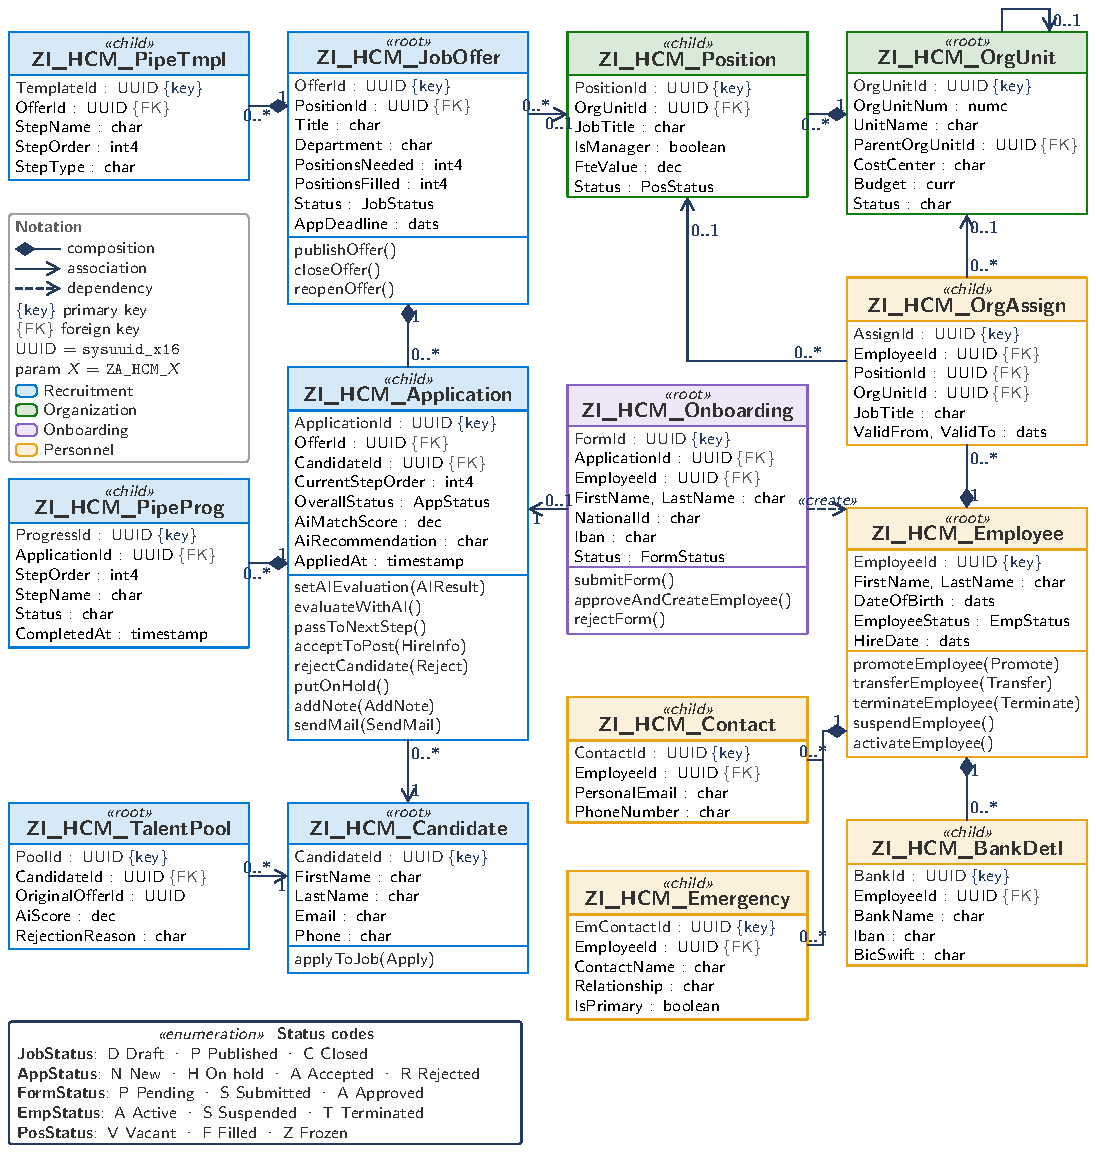
\includegraphics[width=\textwidth]{Figures/class_diagram.pdf}
    \caption{Class Diagram of the Talently Data Model (CDS Interface Views)}
    \label{fig:class_diagram}
\end{figure}

Each class is a CDS interface view (\code{ZI_HCM_*}) showing its main fields and its RAP actions, colored by domain. Three types of relationships are used:

\begin{itemize}
    \item \textbf{Composition} (filled diamond): the child is created, locked, and deleted with its parent (1 to 0..*): job offer to pipeline steps and applications, application to progress records, organizational unit to positions, and employee to contact, bank, emergency, and assignment records.
    \item \textbf{Association} (arrow): a link between independent objects: application to candidate (0..* to 1), onboarding form to application (0..1 to 1), job offer to position (0..* to 0..1), talent-pool entry to candidate, assignment to position and organizational unit, and organizational unit to its parent unit (0..1).
    \item \textbf{Dependency} (dashed arrow): the onboarding form creates the employee through \code{approveAndCreateEmployee}.
\end{itemize}

All keys are UUIDs, the \{FK\} fields implement the associations, and the status codes are listed in the enumeration box.

% ─────────────────────────────────────────────
\section*{Conclusion}
\addcontentsline{toc}{section}{Conclusion}
% ─────────────────────────────────────────────

This chapter presented the design of Talently. The global architecture separates the SAP BTP backend, which holds all business data and rules, from the AI microservice and the two user interfaces. The RAP backend was described through its layers, business objects, actions, and transaction model, and the AI engine through its six-stage pipeline and scoring rubric. The sequence diagrams, the routing tree, and the class diagram detailed the main scenarios and the data model. The next chapter presents the tools used to build the solution, demonstrates it end to end, and evaluates it.

\fussy
